\documentclass[crop,tikz]{standalone}% 'crop' is the default for v1.0, before it was 'preview'
\usepackage{tikz,calc,pgfplots}
\usetikzlibrary{calc,patterns}
\begin{document}


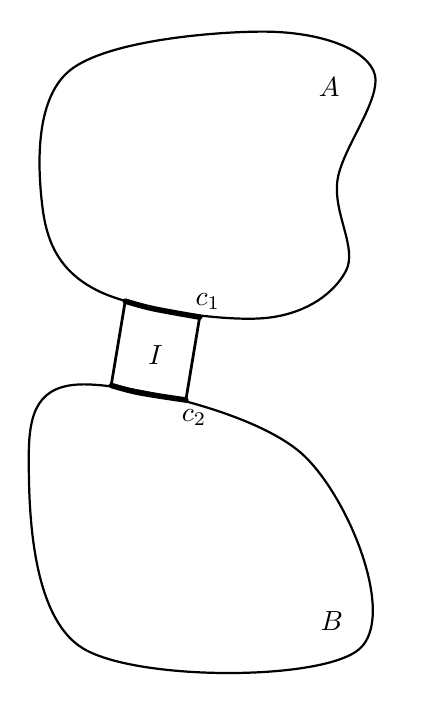
\begin{tikzpicture}[scale = 0.7]

\begin{scope}[shift={(0.25,1.5)}]

 \draw [thick]  plot[smooth cycle, tension=.6] coordinates {(0,2) (0.5,4.5) (4,5.2) (6,4.5)  (5.35,2.5) (5.5,0.85) (4,0) (1,0.5) };
\node[outer sep=0pt,thick] at (5.2,4.2) [minimum width=1.5cm, minimum height=1.5cm] {${A}$};
 
%\draw [thick,dashed, fill=white!70!black]  plot[smooth cycle,  tension=.6] coordinates {(1.5,2.8) (1.5,4) (2.5,4)  (2.5,3.2) };

%\node[outer sep=0pt,thick] at (2,3.5) [minimum width=1.5cm, minimum height=1.5cm] {$o$};
 
 
 % \draw [line width=2pt,black,cap=round]  plot[smooth, tension=.6] coordinates { (3.25,5.175) (4,5.2) (4.75,5.15) };  
 % \node[outer sep=0pt,thick] at (4,5.5) [minimum width=1.5cm, minimum height=1.5cm] {$a$};
 
 \draw [line width=2pt,black,cap=round]  plot[smooth, tension=.6] coordinates { (2.85,0.02) (2,0.175) (1.5,0.31) };  
 \node[outer sep=0pt,thick] at (3,0.3) [minimum width=1.5cm, minimum height=1.5cm] {$c_1$};
 
 \end{scope}
 
\draw [line width=1pt,black,cap=round]  plot[smooth, tension=.6] coordinates { (2.85,0.016) ($(2.85,0.02) + (0.25,1.5)$) };  
\draw [line width=1pt,black,cap=round]  plot[smooth, tension=.6] coordinates { (1.5,0.31)  ($(1.5,0.31) + (0.25,1.5)$) };  
\node[outer sep=0pt,thick] at ($(2,0.175)+ (0.3,0.65)$) [minimum width=1.5cm, minimum height=1.5cm] {${I}$}; 
 
  \draw [line width=2pt,black,cap=round]  plot[smooth, tension=.6] coordinates { (2.85,0.016) (2,0.15) (1.5,0.28) };  
 \node[outer sep=0pt,thick] at (3,-0.3) [minimum width=1.5cm, minimum height=1.5cm] {$c_2$};
 
\draw [thick]  plot[smooth cycle, tension=.6] coordinates {(0,-1) (1,-4.5) (6,-4.5) (5,-1) (1,0.3) };
\node[outer sep=0pt,thick] at (5.5,-4) [minimum width=1.5cm, minimum height=1.5cm] {${B}$};


%\draw [line width=2pt,black,cap=round]  plot[smooth, tension=.6] coordinates {  (0.045,-0.5) (0.025,-1.5) (0.03,-2) };  
%\node[outer sep=0pt,thick] at (0.4,-1.3) [minimum width=1.5cm, minimum height=1.5cm] {$b$}; 


% \draw [line width=2pt,black,cap=round]  plot[smooth, tension=.6] coordinates {  (6,-4.5) (5.2,-4.8) (4.5,-4.9) };  
% \node[outer sep=0pt,thick] at (5.5,-5.2) [minimum width=1.5cm, minimum height=1.5cm] {$r$};

 \end{tikzpicture}
\end{document}